\documentclass[11pt,a4paper]{article}

\usepackage{geometry}
\geometry{legalpaper, margin=1in}

\usepackage[utf8]{inputenc}
\usepackage[T1]{fontenc}
\usepackage{amsmath,amssymb,amsfonts}
\usepackage{graphicx}
\usepackage{float}
\usepackage{hyperref}
\usepackage{xcolor}
\usepackage{caption}
\usepackage{subcaption}

\title{Methods in Computational Neuroscience\\
Single Neuron Modeling: Action Potential Generation}
\author{Sepehr SAEEDPOUR}
\date{\today}

\begin{document}

\maketitle

\section*{Introduction}

The Integrate-and-Fire model, first conceptualized by Louis Lapicque in 1907, emerged as one of the earliest mathematical frameworks for understanding neuronal activity. This pioneering approach represented neurons as simple electrical circuits capable of accumulating charge until reaching a threshold, at which point a spike would occur. For decades, this abstraction served as the primary computational description of neural function, until Alan Hodgkin and Andrew Huxley's revolutionary work in the early 1950s. Through meticulous experiments on the giant squid axon, for which they later received the Nobel Prize, Hodgkin and Huxley revealed the ionic basis of action potentials and developed their eponymous model that explained spike generation through the coordinated dynamics of voltage-gated sodium and potassium channels. These two models represent pivotal moments in the history of computational neuroscience, marking the evolution from phenomenological descriptions to mechanistic explanations of neural activity.

In this assignment, we implement and analyze both models to explore how neurons generate action potentials in response to various stimuli. For the Integrate-and-Fire neuron, we examine membrane potential dynamics using numerical and analytical methods, investigating how the model responds to different current intensities, noise levels, and time-varying inputs. We characterize the relationship between input strength and firing rate, demonstrating how information might be encoded in spike frequency. Our simulations reveal the model's capacity to transform continuous signals into discrete spike trains, highlighting fundamental principles of neural coding.

We then investigate the more biophysically detailed Hodgkin-Huxley model, focusing on how the interplay between sodium and potassium conductances gives rise to the characteristic shape and properties of action potentials. By varying the input current, we identify distinctive features absent in simpler models, such as the existence of a minimum firing rate and the complex dynamics near threshold. Through these comparative analyses, we gain insight into how neurons integrate inputs and generate outputs, contributing to our understanding of information processing in the nervous system. This exploration demonstrates how computational modeling serves as a powerful tool for investigating neural function across different levels of abstraction

\section{Integrate-and-Fire Neuron}

\subsection{Simulating Membrane Potential Dynamics}

The passive membrane potential dynamics of a neuron are described by the following differential equation:
\begin{equation}
C \frac{dV(t)}{dt} = g_L(E_L - V(t)) + I
\end{equation}

where $C = 1\mu F$ is the membrane capacitance, $g_L = 0.1\mu S$ is the conductance of the membrane, and $E_L = -70mV$ is the reversal potential. To solve this equation numerically, I implemented the Euler method:
\begin{equation}
V(t + \Delta t) = V(t) + \frac{dV(t)}{dt} \Delta t
\end{equation}

Figure 1 shows the membrane potential evolution with $I = 1nA$, initial condition $V(0) = E_L$, and time step $\Delta t = 1ms$ over 100ms.

\begin{figure}[H]
\centering
% Insert Figure 1: Membrane potential with I=1nA
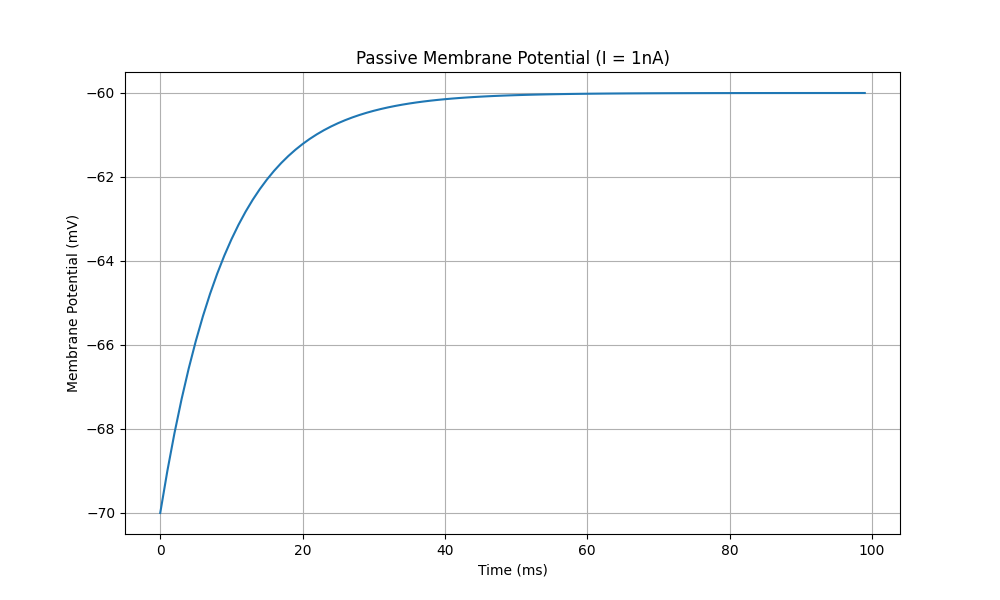
\includegraphics[width=0.7\textwidth]{fig1.png}

\caption{Membrane potential of a passive neuron with $I = 1nA$. The potential rises from the resting value $E_L = -70mV$ and approaches a steady state.}
\label{fig:passive_membrane}
\end{figure}

\subsection{Effect of Current Variation}

The membrane potential with different current values is simulated (Figure 2). As the injected current increases, the membrane potential rises more quickly and reaches a higher steady-state value. This is expected from the differential equation, as a larger $I$ creates a stronger drive away from the reversal potential.

\begin{figure}[H]
\centering
% Insert Figure 2: Membrane potential with different currents
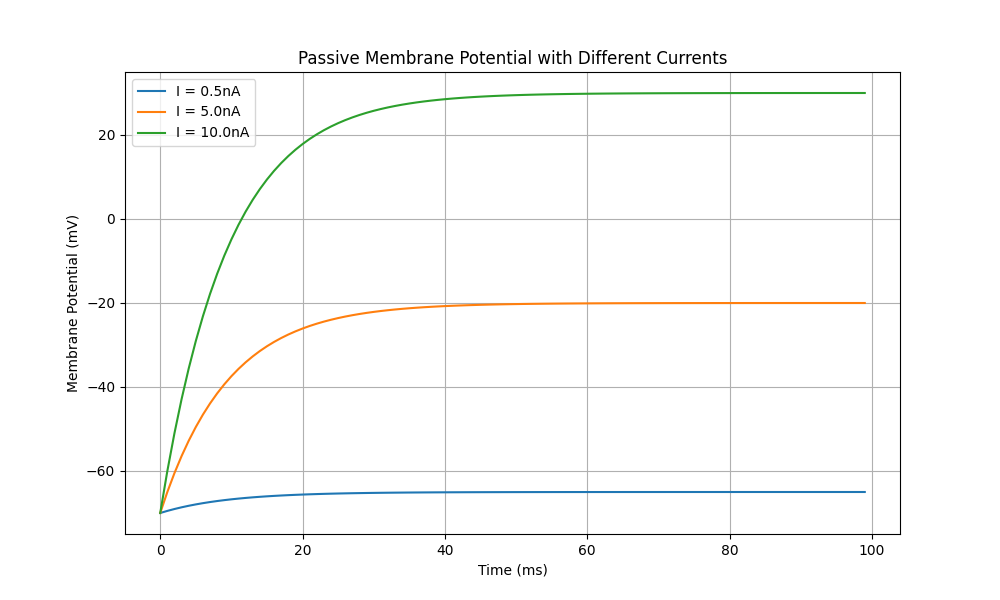
\includegraphics[width=0.7\textwidth]{fig2.png}
\caption{Membrane potential dynamics with different injected currents. Higher currents lead to faster rises and higher steady-state values.}
\label{fig:current_variation}
\end{figure}

% \subsection{Analytical Solution}
\subsection{Solve the ODE}

The passive membrane equation describes how the membrane potential $V(t)$ evolves over time in response to an input current $I$:

\begin{equation}
C \frac{dV(t)}{dt} = g_L(E_L - V(t)) + I
\end{equation}

To derive the analytical solution, I first rearrange this equation into standard form:

\begin{equation}
\frac{dV(t)}{dt} = \frac{g_L}{C}(E_L - V(t)) + \frac{I}{C}
\end{equation}

This is a first-order linear differential equation of the form $\frac{dy}{dt} + P(t)y = Q(t)$, where $P(t) = \frac{g_L}{C}$ and $Q(t) = \frac{g_L E_L + I}{C}$. The general solution is given by:

\begin{equation}
y = e^{-\int P(t) dt} \left[ \int Q(t) e^{\int P(t) dt} dt + K \right]
\end{equation}

where $K$ is a constant determined by the initial conditions.

For our equation, $\int P(t) dt = \frac{g_L}{C}t$, so $e^{\int P(t) dt} = e^{\frac{g_L}{C}t}$.

Substituting into the general solution:

\begin{equation}
V(t) = e^{-\frac{g_L}{C}t} \left[ \int \frac{g_L E_L + I}{C} e^{\frac{g_L}{C}t} dt + K \right]
\end{equation}

Computing the integral:

\begin{equation}
\int \frac{g_L E_L + I}{C} e^{\frac{g_L}{C}t} dt = \frac{g_L E_L + I}{g_L} e^{\frac{g_L}{C}t} + C_1
\end{equation}

where $C_1$ is a constant of integration. Therefore:

\begin{equation}
V(t) = e^{-\frac{g_L}{C}t} \left[ \frac{g_L E_L + I}{g_L} e^{\frac{g_L}{C}t} + K \right]
\end{equation}

Simplifying:

\begin{equation}
V(t) = \frac{g_L E_L + I}{g_L} + K e^{-\frac{g_L}{C}t}
\end{equation}

Using the initial condition $V(0) = E_L$, we find:

\begin{equation}
E_L = \frac{g_L E_L + I}{g_L} + K
\end{equation}

Solving for $K$:

\begin{equation}
K = E_L - \frac{g_L E_L + I}{g_L} = -\frac{I}{g_L}
\end{equation}

Therefore, the final analytical solution is:

\begin{equation}
V(t) = \frac{g_L E_L + I}{g_L} - \frac{I}{g_L} e^{-\frac{g_L}{C}t} = E_L + \frac{I}{g_L} (1 - e^{-\frac{g_L}{C}t})
\end{equation}

We can define the time constant $\tau = \frac{C}{g_L}$ and the steady-state potential $V_{\infty} = E_L + \frac{I}{g_L}$, leading to the commonly used form:

\begin{equation}
V(t) = E_L + (V_{\infty} - E_L) (1 - e^{-\frac{t}{\tau}})
\end{equation}

To validate the numerical implementation, the Euler method is compared with the analytical solution derived above. Using the parameters $C = 1\mu F$, $g_L = 0.1\mu S$, $E_L = -70mV$, and $I = 1nA$. 

The membrane time constant for these parameters is $\tau = \frac{C}{g_L} = \frac{1\mu F}{0.1\mu S} = 10ms$, indicating that the membrane potential reaches approximately 63\% of its steady-state value after 10ms. The steady-state potential is $V_{\infty} = E_L + \frac{I}{g_L} = -70mV + \frac{1nA}{0.1\mu S} = -60mV$.

Figure 3 shows the comparison between the two solutions along with the absolute and relative errors. The numerical solution using the Euler method with a time step of $\Delta t = 1ms$ closely follows the analytical solution. These small errors confirm the accuracy of the numerical implementation.

\begin{figure}[ht]
    \centering
    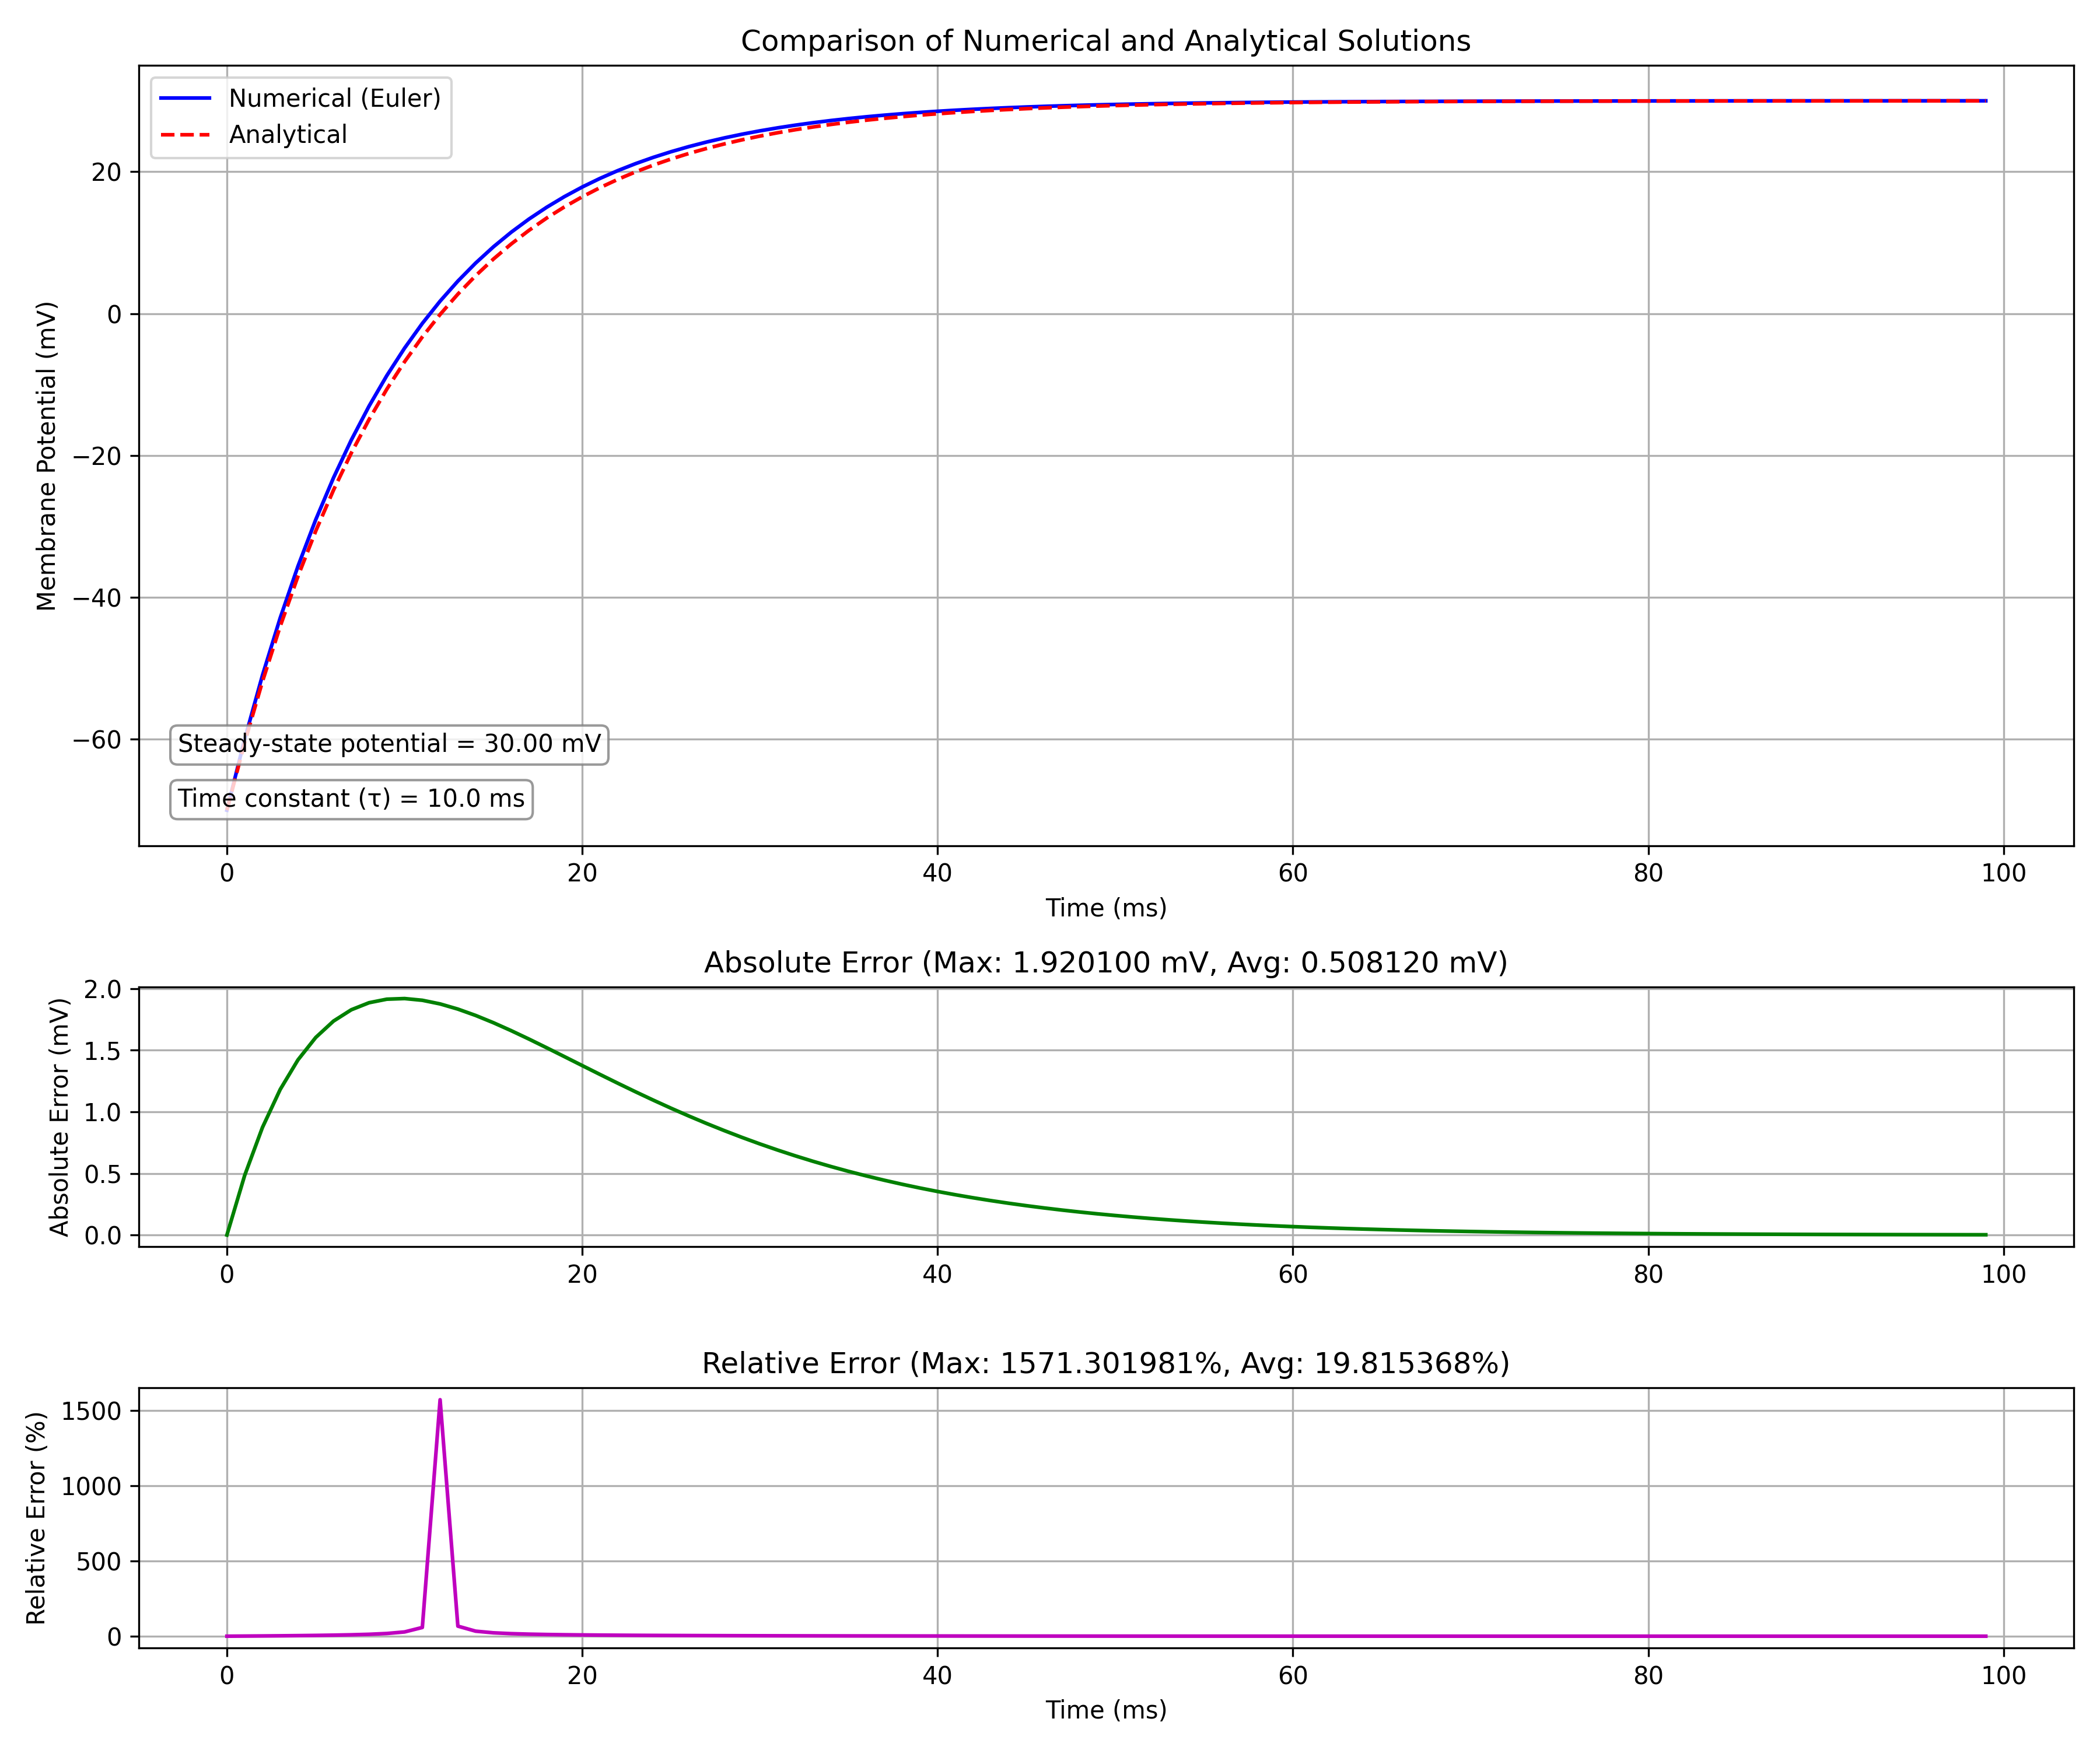
\includegraphics[width=0.7\textwidth]{fig3.png}
    \caption{Detailed comparison between numerical and analytical solutions. (Top) Membrane potential trajectories showing excellent agreement between the Euler method and the exact solution. (Middle) Absolute error in mV as a function of time. (Bottom) Relative error as a percentage of the analytical value. Note that the errors are extremely small, indicating high accuracy of the numerical method with the chosen time step.}
\end{figure}
\pagebreak

The absolute error increases initially as the membrane potential changes quickly, reaches a maximum, and then stabilizes as both solutions approach the steady state. This behavior is expected since the Euler method approximates the derivative at the beginning of each time step, leading to a slight lag in tracking fast changes in the solution.


The agreement between the analytical and numerical solutions confirms that the implementation is correct and provides an evidence for usability of this method, where analytical solutions are either unavailable or difficult to derive (e.g., in the Hodgkin Huxley model).




\subsection{Spiking Mechanism}

A spiking mechanism is implemented where the neuron fires an action potential when the membrane potential exceeds a threshold $V_{th} = -63mV$. The spike is represented by setting the voltage to $V_{max} = +30mV$, followed by a reset to $E_L = -70mV$.

The implementation follows:
\begin{equation}
\text{If } V(t) \geq V_{th} \text{, then: }
\begin{cases}
V(t) = V_{max} \\
V(t+\Delta t) = E_L
\end{cases}
\end{equation}

Figure 4 shows the membrane potential with this spiking mechanism.

\begin{figure}[H]
\centering
% Insert Figure 4: Membrane potential with spiking mechanism
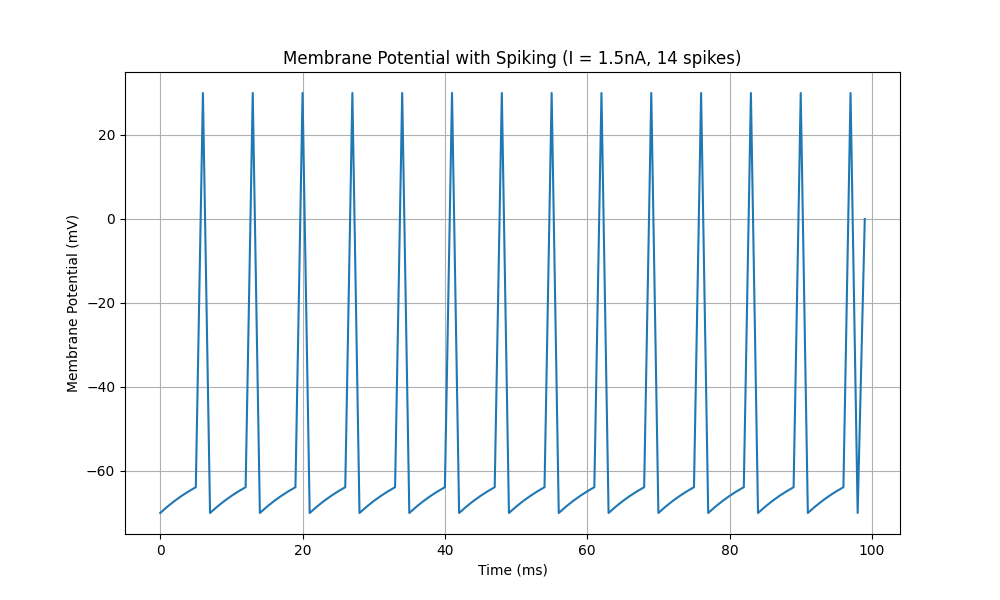
\includegraphics[width=0.7\textwidth]{fig4.png}
\caption{Membrane potential dynamics with spiking mechanism. When the potential reaches threshold, a spike occurs followed by a reset.}
\label{fig:spiking_mechanism}
\end{figure}

\subsection{How many spikes?}

With $I = 1.5nA$, the neuron produces approximately 14 spikes within 100ms (Fig 4). To determine the relationship between input current and firing rate, the current and counted the resulting spikes are varied.

The neuron begins firing when the input current is sufficient to drive the membrane potential above threshold. From the steady-state solution, this occurs when:
\begin{equation}
E_L + \frac{I}{g_L} \geq V_{th}
\end{equation}

Solving for $I$:
\begin{equation}
I \geq g_L(V_{th} - E_L) = 0.1\mu S \cdot (-63mV - (-70mV)) = 0.7nA
\end{equation}

Figure 5 shows the tuning curve (number of spikes vs. input current).

\begin{figure}[H]
\centering
% Insert Figure 5: Tuning curve
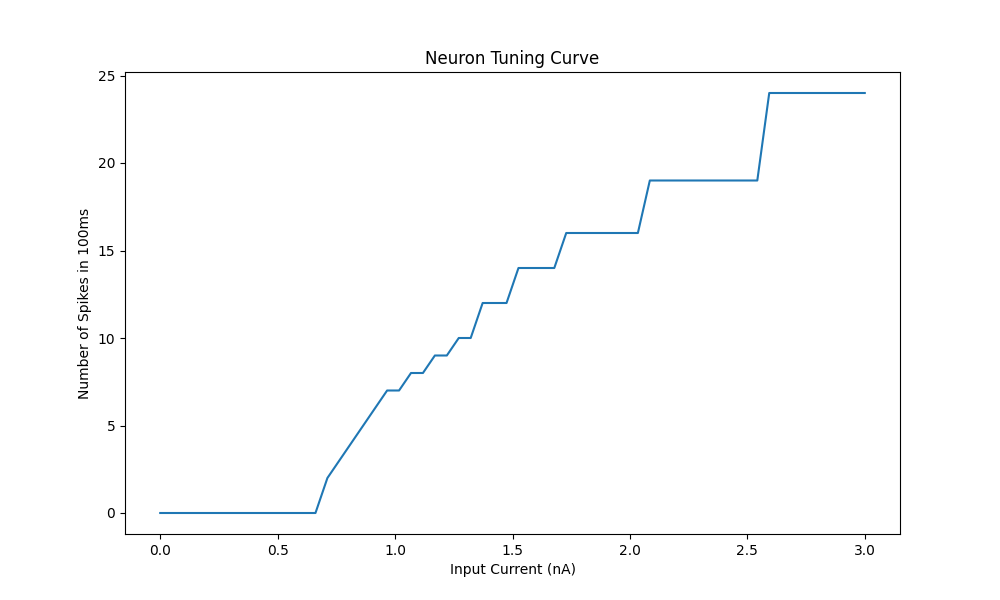
\includegraphics[width=0.7\textwidth]{fig5.png}
\caption{Tuning curve showing the number of spikes in 100ms as a function of input current. The neuron begins firing at approximately 0.7nA, and the firing rate increases approximately linearly with current.}
\label{fig:tuning_curve}
\end{figure}

The tuning curve appears to have "step-like" intervals where the spike count remains constant despite increasing current. This occurs because of the discrete nature of spike counting in a fixed time window.


When the input current increases gradually, there are ranges where the increase isn't enough to generate an additional action potential within the 100ms observation window. The neuron can only fire a whole number of spikes in the fixed time period, so the spike count must increase in integer steps.

\subsection{Noise and Spike Trains}

To introduce more realistic behavior,a white noise term is added:
\begin{equation}
C \frac{dV(t)}{dt} = g_L(E_L - V(t)) + I + \sigma\eta(t)
\end{equation}

where $\sigma$ controls the noise magnitude and $\eta(t)$ is a random variable from a normal distribution with mean 0 and variance 1. In discrete simulation, the noise term is scaled by $\sqrt{\Delta t}$ to ensure time step independence.

Figure 6 shows membrane potential dynamics with different noise levels.

\begin{figure}[H]
\centering
% Insert Figure 6: Membrane potential with noise
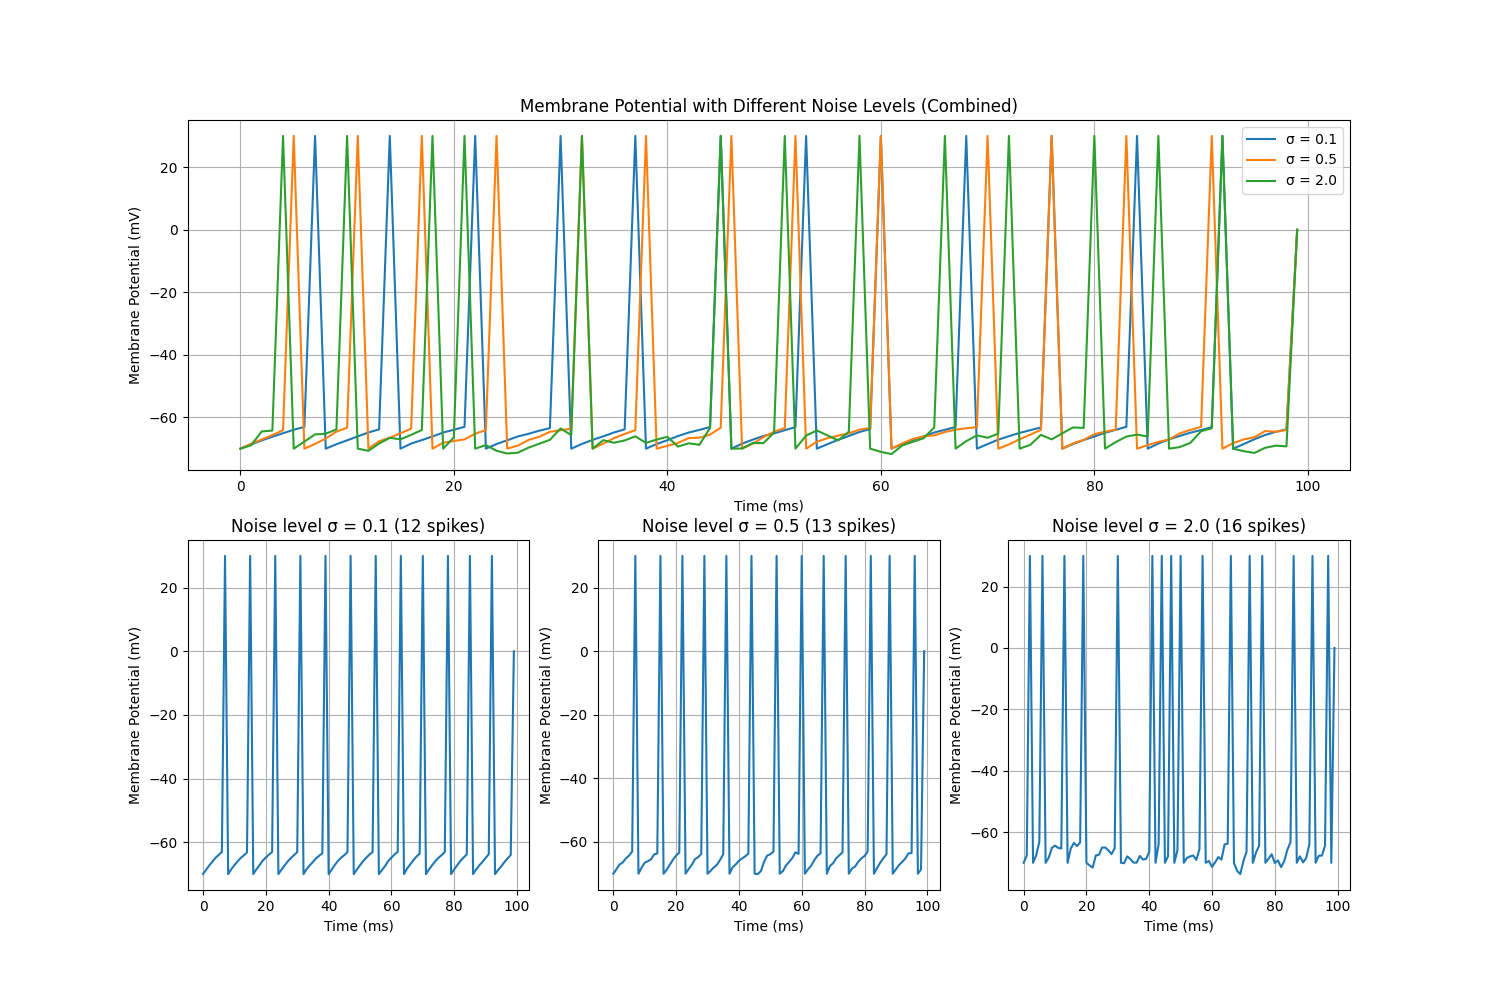
\includegraphics[width=0.7\textwidth]{fig6.png}
\caption{Membrane potential dynamics with different noise levels. Higher noise introduces greater variability and can cause spontaneous spiking.}
\label{fig:noise_effects}
\end{figure}

With low noise ($\sigma = 0.1$), small fluctuations appear in the membrane potential, but the overall spiking pattern remains similar to the deterministic case. With medium noise ($\sigma = 0.5$), the spike timing becomes variable, and occasionally extra spikes occur. With high noise ($\sigma = 2.0$), substantial variability is observed, including spontaneous spikes that would not occur in the deterministic model.

\subsection{Time-varying Input}

A time-varying input by defining $I(t)$ as a pulse:
\begin{equation}
I(t) = 
\begin{cases}
3 - \frac{t}{10}, & \text{if } 10 \leq t < 40 \\
1.5 + \eta_t, & \text{if } 65 \leq t < 85 \\
0 & \text{otherwise}
\end{cases}
\end{equation}
where $\eta_t \sim \mathcal{N}(0, 0.5)$ represents Gaussian noise with mean 0 and standard deviation 0.5.


Figure 7 shows the membrane potential response to this time-varying input, along with low-level noise.

\begin{figure}[H]
\centering
% Insert Figure 7: Response to time-varying input
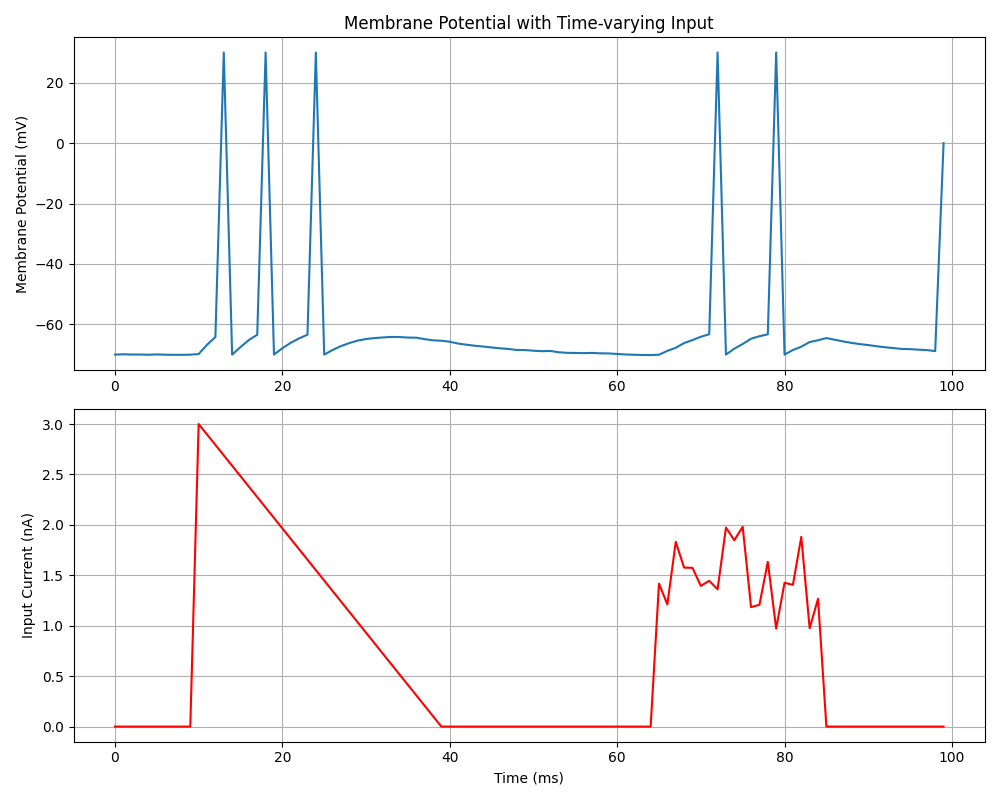
\includegraphics[width=0.7\textwidth]{fig7.png}
\caption{Membrane potential (top) in response to a time-varying input current (bottom). Spikes occur during the period when the current is on.}
\label{fig:time_varying}
\end{figure}

The neuron spikes repetitively during the period when the input current is on, demonstrating how neurons can encode temporal patterns in their input. The addition of low-level noise makes the response more realistic, with slight variations in spike timing.

\section{Hodgkin-Huxley Model}

\subsection{HH Dynamics}

The Hodgkin-Huxley model describes action potential generation through voltage-dependent ion channels. The membrane potential dynamics are governed by:
\begin{equation}
C \frac{dV}{dt} = g_L(E_L - V) + \bar{g}_K n^4(E_K - V) + \bar{g}_{Na}m^3h(E_{Na} - V) + I
\end{equation}

The channel variables $n$, $m$, and $h$ follow first-order kinetics:
\begin{equation}
\frac{dx}{dt} = \alpha_x(V)(1 - x) - \beta_x(V)x
\end{equation}

where $x$ represents any of the gating variables, and $\alpha_x(V)$ and $\beta_x(V)$ are voltage-dependent opening and closing rates.

I implemented the model with parameters: $C = 1\mu F/cm^2$, $g_L = 0.3mS/cm^2$, $E_L = -54.4mV$, $g_K = 36mS/cm^2$, $E_K = -77mV$, $g_{Na} = 120mS/cm^2$, and $E_{Na} = 50mV$.

Figure 8 shows the dynamics of $V$, $n$, $m$, and $h$ with $I = 10nA$.

\begin{figure}[H]
\centering
% Insert Figure 8: HH dynamics
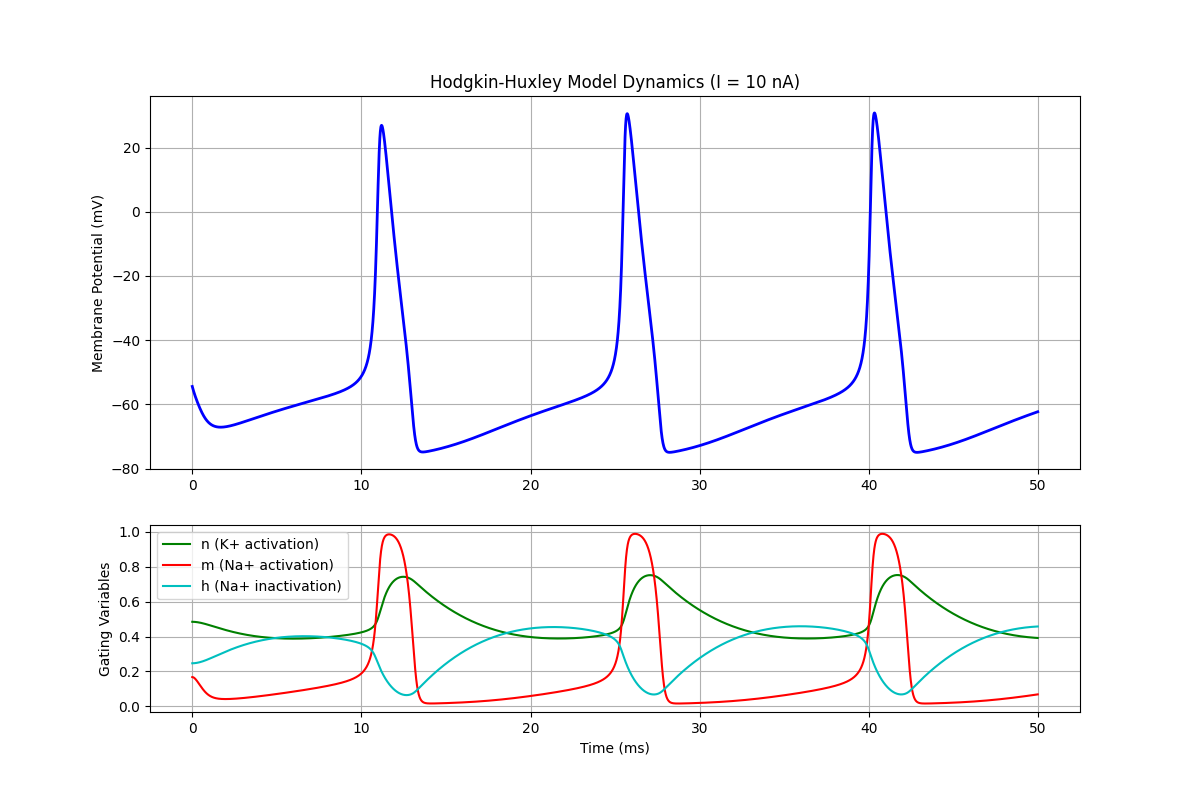
\includegraphics[width=0.7\textwidth]{fig8.png}
\caption{Hodgkin-Huxley model dynamics with $I = 10nA$. Top: Membrane potential showing action potentials. Bottom: Gating variables $n$ (K$^+$ activation), $m$ (Na$^+$ activation), and $h$ (Na$^+$ inactivation).}
\label{fig:hh_dynamics}
\end{figure}

The simulation reveals the interactions between different ion channels during action potential generation.
$m$ rises fast during the spike onset, allowing Na$^+$ influx and depolarization.
$h$ decreases during the spike, inactivating Na$^+$ channels. Finally,
$n$ rises slowly, activating K$^+$ channels and repolarizing the membrane.

\subsection{Vary I (Current)}

The injected current is varied from $I = 0nA$ to $I = 15nA$ to determine the spiking threshold. Figure 9 shows the number of spikes in 200ms as a function of input current.

\begin{figure}[H]
\centering
% Insert Figure 9: HH firing rate vs. current
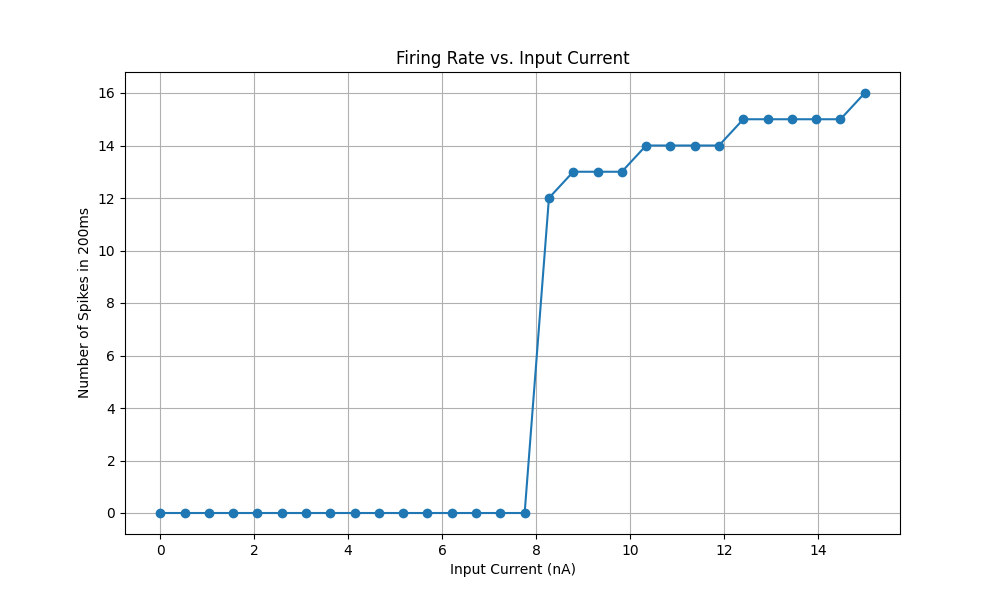
\includegraphics[width=0.7\textwidth]{fig9.png}
\caption{Number of spikes in 200ms as a function of input current for the Hodgkin-Huxley model.}
\label{fig:hh_firing_rate}
\end{figure}

The neuron begins to spike repetitively at approximately $I = 8.3nA$. Unlike the integrate-and-fire model, which can fire at arbitrarily low frequencies, the Hodgkin-Huxley model exhibits a minimum firing rate of approximately (50 Hz) at threshold. 

Figure 10 shows the membrane potential dynamics at currents just below, at, and above threshold.

\begin{figure}[H]
\centering
% Insert Figure 10: HH near threshold behavior
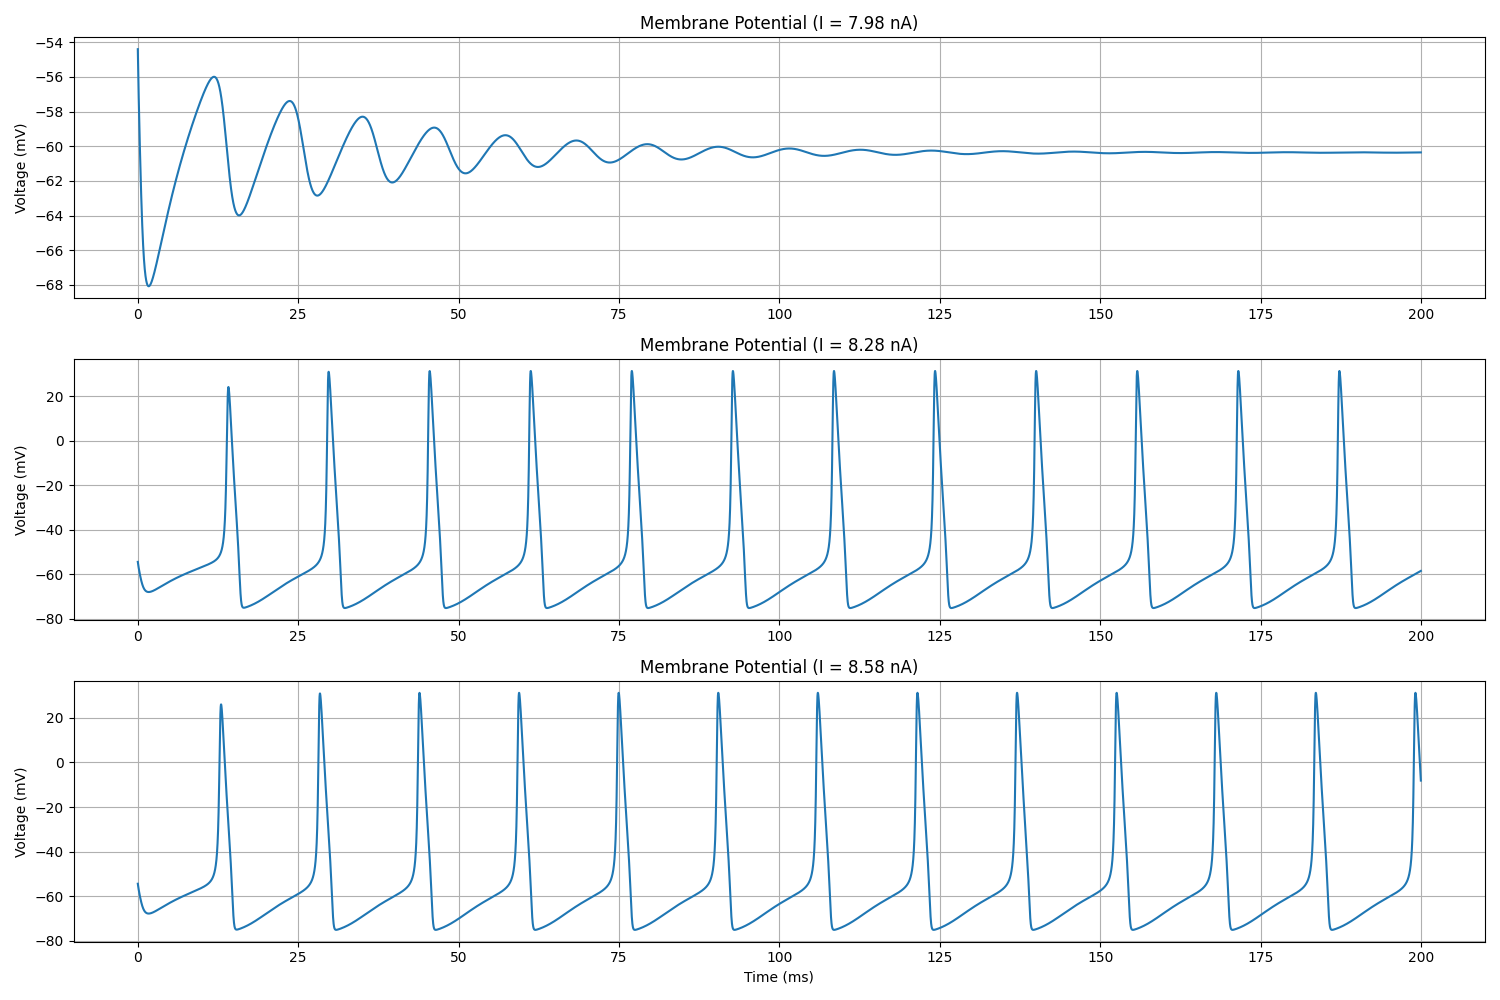
\includegraphics[width=0.7\textwidth]{fig10.png}
\caption{Membrane potential dynamics with currents near threshold. Top: Below threshold - single spike or no spikes. Middle: At threshold - delayed regular spiking. Bottom: Above threshold - regular spiking with higher frequency.}
\label{fig:hh_threshold}
\end{figure}

At threshold, the HH model shows a characteristic delay before spiking begins, and then maintains a regular firing pattern. This contrasts with the integrate-and-fire model, which begins firing as soon as the threshold is reached. The difference arises from the complex interactions between activation and inactivation dynamics of the ion channels in the HH model.

\section*{Conclusion}

This assignment explored two fundamental models of neuronal action potential generation. The integrate-and-fire model provides a simplified representation that captures basic spiking behavior, while the Hodgkin-Huxley model offers deeper insights into the biophysical mechanisms underlying action potentials.

Key findings include:
\begin{itemize}
\item In both models, increasing input current leads to increased firing rates (Figure 5 and 9)
\item The integrate-and-fire model shows a gradual onset of spiking (Figure 5)
\item The Hodgkin-Huxley model exhibits an abrupt onset of repetitive firing with a minimum frequency (Figure 9 and 10)
\item Noise introduces variability in spike timing, making the models more biologically realistic (Figure 6)
\item Time-varying inputs demonstrate how neurons can encode temporal information in their spike patterns (Figure 7)
\end{itemize}

These simulations highlight the mechanisms by which neurons transform continuous input signals into discrete spike trains, forming the basis for information processing in the nervous system.

\end{document}